\section{Results\label{sec:results}}

%###################################################################
%#    Weak Scaling on Stampede2, Laplace kernel, 1e7 points/node   # 
%###################################################################
%===========================================================================================
%|Nodes      Dist | TotalTime  InitTree  InitFMM_Tree  SetupFMM  RunFMM (GFlop/s)  Scatter | 
%===========================================================================================
%|    1      Unif |     3.766     0.530         0.189     0.120    2.808 (590.7)     0.100 |
%|    2      Unif |     2.883     0.757         0.246     0.346    1.320 (556.4)     0.125 |
%|    4      Unif |     3.340     0.740         0.217     0.354    1.822 (559.4)     0.129 |
%|    8      Unif |     4.517     0.741         0.199     0.274    3.104 (560.7)     0.132 |
%|   16      Unif |     3.516     1.041         0.250     0.507    1.437 (524.9)     0.195 |
%|   32      Unif |     3.861     1.008         0.236     0.439    1.909 (542.4)     0.188 |
%|   64      Unif |     5.140     1.112         0.204     0.377    3.161 (560.1)     0.212 |
%|  128      Unif |     4.218     1.563         0.253     0.538    1.487 (512.8)     0.286 |
%===========================================================================================
%|    1  Non-unif |     2.966     0.796         0.240     0.246    1.511 (555.9)     0.097 |
%|    2  Non-unif |     3.257     0.853         0.247     0.249    1.710 (525.6)     0.124 |
%|    4  Non-unif |     3.424     0.929         0.266     0.297    1.719 (493.8)     0.135 |
%|    8  Non-unif |     4.129     1.033         0.303     0.373    2.180 (410.3)     0.152 |
%|   16  Non-unif |     4.499     1.151         0.403     0.393    2.290 (373.1)     0.168 |
%|   32  Non-unif |     4.862     1.361         0.461     0.415    2.337 (383.2)     0.188 |
%|   64  Non-unif |     5.695     1.539         0.804     0.462    2.575 (332.3)     0.213 |
%|  128  Non-unif |     5.818     1.701         0.877     0.430    2.483 (360.6)     0.222 |
%===========================================================================================
%
%###################################################################
%#    Strong Scaling on Stampede2, Laplace kernel, 1e8 points      # 
%###################################################################
%===========================================================================================
%|Nodes      Dist | TotalTime  InitTree  InitFMM_Tree  SetupFMM  RunFMM (GFlop/s)  Scatter | 
%===========================================================================================
%|    1      Unif |    30.002     7.964         2.312     2.454   15.216 (570.9)     1.201 |
%|    2      Unif |    15.802     4.457         1.254     1.366    7.640 (568.7)     0.628 |
%|    4      Unif |     8.385     2.299         0.682     0.827    3.987 (545.0)     0.372 |
%|    8      Unif |     4.549     1.170         0.438     0.570    2.077 (523.4)     0.189 |
%|   16      Unif |     2.530     0.615         0.293     0.373    1.098 (495.5)     0.097 |
%|   32      Unif |     1.373     0.337         0.172     0.211    0.588 (463.0)     0.047 |
%|   64      Unif |     0.747     0.187         0.094     0.120    0.317 (430.1)     0.026 |
%|  128      Unif |     0.500     0.109         0.061     0.082    0.226 (303.1)     0.019 |
%===========================================================================================
%|    1  Non-unif |    31.260     9.059         2.421     2.330   15.475 (571.5)     1.196 |
%|    2  Non-unif |    16.585     5.063         1.269     1.102    8.052 (549.6)     0.664 |
%|    4  Non-unif |     8.899     2.552         0.650     0.643    4.456 (497.7)     0.379 |
%|    8  Non-unif |     5.191     1.382         0.380     0.462    2.668 (417.0)     0.183 |
%|   16  Non-unif |     2.805     0.710         0.188     0.304    1.453 (384.8)     0.098 |
%|   32  Non-unif |     1.623     0.391         0.116     0.196    0.845 (333.7)     0.051 |
%|   64  Non-unif |     0.917     0.236         0.070     0.098    0.479 (297.4)     0.028 |
%|  128  Non-unif |     0.566     0.118         0.048     0.077    0.301 (239.7)     0.020 |
%===========================================================================================

In this section, we present scalability results for our blood flow simulation
framework on various test geometries, simulations with various volume fractions 
and demonstrate the convergence behavior of our numerical methods.
%We also highlight simulations with various volume fractions,
%including one with volume fraction comparable to realistic human blood 
%flows.

\begin{figure}[!th]
\centering
%\resizebox{.5\columnwidth}{!}{%
\begin{minipage}[b]{0.48\textwidth}
\begin{tikzpicture}[scale=0.7] %<<<
  \begin{semilogxaxis}[
    scale only axis,
    axis lines=left,
    xtick=data,
    xticklabels={384,768,1536,3072,6144,12288},
    ybar stacked,
    legend style={
      draw=none,
      at={(0.42,1.0)},
      anchor=north,
      legend columns=3,
      /tikz/every even column/.append style={column sep=0.5cm}},
    legend entries={\bf COL, \bf BIE-solve, \bf BIE-FMM, \bf
      Other-FMM, \bf Other},
    xlabel=\cpu cores $\rightarrow$,
    ytick={0,2000000,4000000,6000000,8000000,1000000},
    ymajorgrids,ylabel=wall-time $\times$ \cpu cores (bar) $\rightarrow$,
%    scaled ticks=base 10:0,
    xmin=250,
    xmax=25600,
    ymin=0,
    ymax=10000000,
    bar width=22pt,
    width=3.8in,
    height=3in]
 
    \addplot[color=black, fill=clr10]
    table[x=cs,y=col] {result_data/strong_result_scaled_detail};

    \addplot[color=black, fill=clr5]
    table[x=cs,y=wsolveother] {result_data/strong_result_scaled_detail};

    \addplot[color=black, fill=clr12]
    table[x=cs,y=wfmm] {result_data/strong_result_scaled_detail};

    \addplot[color=black, fill=clr13]
    table[x=cs,y=otherfmm] {result_data/strong_result_scaled_detail};

    \addplot[color=black, fill=clr14]
    table[x=cs,y=other] {result_data/strong_result_scaled_detail};

  \end{semilogxaxis}
%    \begin{semilogxaxis}[
%        scale only axis,
%      axis lines=right,
%      xtick=data,
%      xticklabels={384, 768,1536, 3072, 6144,12288},
%      axis x line=none,   
%      legend style={
%        draw=none,
%        at={(0.68,.95)},
%        anchor=north,
%        legend columns=3,
%        /tikz/every even column/.append style={column sep=0.5cm}},
%     legend entries={wall-time},
%     xlabel=\cpu cores $\rightarrow$,
%     ytick={0,3000,6000,9000,12000},
%     ylabel=wall-time (plot) $\rightarrow$,
%     %ymajorgrids,ylabel=wall-time $\rightarrow$,
% %    scaled ticks=base 10:0,
%     xmin=250,
%     xmax=25600,
%     ymin=0,
%     ymax=12000,
%     %bar width=22pt,
%     width=3.8in,
%      height=3in]
%    \addplot[color=black,mark=*] table [x=cs,y=walltime]{result_data/strong_result_scaled_detail};
%    \end{semilogxaxis}
%  \node[draw=none] at (4,6.5) {(strong)};
\end{tikzpicture} %>>>
\end{minipage}
\vfill
\begin{minipage}[b]{0.48\textwidth}
    %\begin{table}
        \centering
        \begin{tabular}{ccccccc}\toprule
            cores  \!\!\!\!\!\!\!\!\!     &\!\!\! $384$ \!\!\! & $768$  & \!\!$1536$ & \!\!$3072$ &
            $6144$ & \!\!\! $12288$ \\ \cmidrule(lr){1-1} \cmidrule(lr){2-7}
            total time (sec)  & $11257$ & $5751$ & $3268$ & $1887$ & $1116$ & $718$ \\ 
            efficiency  & $1.00$  & $0.98$ & $0.86$ & $0.75$ & $0.63$ & $0.49$ \\ \hline
            {\bf COL}+{\bf BIE-solve} (sec)  & 3901  & 1843 & 1046 & 596  & 317  & 183 \\
            efficiency & 1.00  & 1.05 & 0.93 & 0.82 & 0.77 & 0.66 \\ \bottomrule
\end{tabular}
    %\end{table}
\end{minipage}
%}
\mcaption{fig:sscale}{
  Strong scalability of a simultion with $40960$ \rbcs on Stampede's
  \abbrev{SKX} partition
  for the vessel network geometry shown in \cref{fig:strong-scale-domain}.}{ The
  vessel is discretized with $40960$ polynomial patches. Shown in the bar graph
  is a breakdown of 
  the compute resources (wall-time $\times$ CPU cores) required by the
  individual components for a simulation with 10 time
  steps on 384 to 12288 cores. The compute resources used by the main algorithms presented in this
  paper are {\bf\em COL} (collision handling), {\bf\em BIE-solve}
  (computation of $\vu^{\Gamma}$, not including FMM calls). Shown in different gray scales are the
  compute resources required by FMM ({\bf\em BIE-FMM} and {\bf\em
    Other-FMM}) and other operations ({\bf\em Other}). Shown in the table
  are the compute time and the parallel efficiency for the
  overall computation and for the sum of {\bf\em COL} and {\bf\em
    BIE-solve}. For the collision avoidance and the
  boundary solve we observe a parallel efficiency of $66$\% for a
  32-fold increase from 384 to 12288 CPU cores.
%    Each vesicle is discretized with spherical harmonic order $16$, 
%    the upsample spherical harmonic order is set to $32$ for inter-particale 
%    potential evaluation and collision detection.
%    The number of total coarse patches on vessel boundary is $10240 \times 4$, 
%    each with $11\times11$ points as sample points.
%    The number of refined patches for quadrature evaluation is $10240 \times 16$,
%    each with $11\times11$ points. Each side has $6$ \abbrev{QBKIX} points.
}
\end{figure}
\subsection{Implementation and example setup}\label{ss:implementation}

\textbf{Architecture and software libraries. } We use the Stampede2 system at the Texas Advanced Computing Center (\abbrev{TACC})
to study the scalability of our algorithms and implementation.
Stampede2 has two types of compute nodes, the Knights Landing (\abbrev{KNL}) compute nodes
and the Skylake (\abbrev{SKX}) compute nodes.
The \abbrev{SKX} cluster has 1,736 dual-socket compute nodes, each with two
24-core 2.1\abbrev{GHz} \cpu{s} and 192\abbrev{GB} of memory.
The \abbrev{KNL} cluster has 4,200 compute nodes, with a 68-core Intel Xeon Phi
7250 1.4\abbrev{Ghz} \cpu{s} and 96\abbrev{GB} of memory plus 16\abbrev{GB} of
high-speed MCDRAM.
We run our simulations in a hybrid distributed-shared memory fashion: we run one
\abbrev{MPI} process per node, with one OpenMP thread per hardware core.
Our largest simulations use 256 \abbrev{SKX} and 512 \abbrev{KNL} nodes.

We leverage several high-performance libraries in our implementation.
We use \abbrev{PETSc}'s \cite{balay2017petsc} parallel matrix and vector operations, and its
parallel \gmres solver. 
Management and distribution of patches describing the blood vessel
geometry uses the \p4est library \cite{BursteddeWilcoxGhattas11}, and
we use \pvfmm
\cite{malhotra2015} for parallel \fmm evaluation.
We also heavily leverage \texttt{Intel MKL} for fast dense linear algebra
routines at the core of our algorithms and \texttt{paraview} for our
visualizations.

\begin{figure}[!htb]
\centering
\begin{minipage}[b]{0.48\textwidth}
\begin{tikzpicture}[scale=0.8] %<<<
  \begin{semilogxaxis}[
    axis lines=left,
    xtick=data,
    xticklabels={48,192,768,3072,12288},
    ybar stacked,
    legend style={
      draw=none,
      at={(0.43,1.0)},
      anchor=north,
      legend columns=3,
      /tikz/every even column/.append style={column sep=0.5cm}},
    %legend entries={v2w, wfmmUL, wfmmVL, wfmmOther, wsolveOther, w2v, v2v, vsolve, col, rep, other},
    %legend entries={col, wsolveother, wfmm, other-fmm, other},
    legend entries={\bf COL, \bf BIE-solve, \bf BIE-FMM, \bf
      Other-FMM, \bf other},
    xlabel=\cpu cores $\rightarrow$,
    ytick={0,5000,10000,15000},
    ymajorgrids,ylabel=wall-time $\rightarrow$,
%    scaled ticks=base 10:0,
    xmin=24,
    xmax=25600,
    ymin=0,
    ymax=15000,
    bar width=22pt,
    width=4.05in,
    height=3in]

    \addplot[color=black, fill=clr10]
    table[x=cs,y=col] {result_data/weak_result_large_grain_large_vol};

    \addplot[color=black, fill=clr5]
    table[x=cs,y=wsolveother] {result_data/weak_result_large_grain_large_vol};

    \addplot[color=black, fill=clr12]
    table[x=cs,y=wfmm] {result_data/weak_result_large_grain_large_vol};

    \addplot[color=black, fill=clr13]
    table[x=cs,y=otherfmm] {result_data/weak_result_large_grain_large_vol};

    \addplot[color=black, fill=clr14]
    table[x=cs,y=other] {result_data/weak_result_large_grain_large_vol};

  \end{semilogxaxis}
%  \node[draw=none] at (4,6.5) {(weak)};
\end{tikzpicture} %>>>
\end{minipage}
\vfill
\begin{minipage}[b]{0.48\textwidth}
        \centering
        \begin{tabular}{cccccc}\toprule
            cores           & $48$   & $192$  & $768$  & $3072$ & $12288$ \\ \cmidrule(lr){1-1} \cmidrule(lr){2-6}
            vol fraction    & $19\%$ & $20\%$ & $23\%$ & $26\%$ & $27\%$ \\ 
            \#collision/ \#\rbcs      & $15\%$ & $13\%$ & $17\%$ & $15\%$ & $16\%$ \\ \bottomrule
            total time (sec)  & $7070$ & $8892$ & $10032$ & $10869$ & $12446$  \\ 
            efficiency  & $ - $  & $1.00$ & $0.88$ & $0.81$ & $0.71$ \\ \bottomrule
            {\bf COL}+{\bf BIE-solve} (sec)   & 1461 & 2345 & 2926 & 3222 & 3904 \\
             efficiency & $-$ & 1.00 & 0.80 & 0.73 & 0.60 \\\bottomrule
            %\bie + Collision Efficiency & 1.00 & 0.62 & 0.37 & 0.46 & 0.37 \\\bottomrule
        \end{tabular}
\end{minipage}
\mcaption{fig:wscale-large-grain}{Weak scalability on Stampede's
  \abbrev{SKX} partition with node grain size of $4096$ \rbcs and
  $8192$ polynomial patches per compute node (each node has 48 cores)
  for the vessel geometry shown in
  \cref{fig:wsscale-domain}.}{ Increasing the number of \rbcs and
  boundary patches is realized by decreasing the size of the \rbcs as
  discussed in \cref{ss:weak}.  Shown in the bar graph is a breakdown of
  wall-time spent in individual components for a simulation with 10 time
  steps on 136 to 12288 cores (i.e., 4 to 256 nodes). The explanation
  of the labels used in the legend is detailed in
  \cref{fig:sscale}. Additionally, we show the volume fraction of
  \rbcs for each simulation, as well as the percentage of vesicles
  where the \rbc-\rbc or \rbc-vessel collision prevention is active.
  We report the parallel scalability with respect to 192 cores, as the
  smallest simulation is in a single node and no MPI communication is
  necessary. The largest simulation has 1,048,576 \rbcs and 2,097,152
  polynomial patches and an overall number of 
  3,042,967,552 unknowns per time step.
}
\end{figure}

\begin{figure}[!htb]
\centering
\begin{minipage}[b]{0.48\textwidth}
\begin{tikzpicture}[scale=0.8] %<<<
  \begin{semilogxaxis}[
    axis lines=left,
    xtick=data,
    xticklabels={136, 544, 2176, 8704, 34816},
    ybar stacked,
    legend style={
      draw=none,
      at={(0.43,1.0)},
      anchor=north,
      legend columns=3,
      /tikz/every even column/.append style={column sep=0.5cm}},
    %legend entries={col, wsolveother, wfmm, other-fmm, other},
    legend entries={\bf COL, \bf BIE-solve, \bf BIE-FMM, \bf
      Other-FMM, \bf other},
    xlabel=\cpu cores $\rightarrow$,
    ytick={0,1000,2000,3000,4000,5000,6000,7000},
    ymajorgrids,ylabel=wall-time $\rightarrow$,
%    scaled ticks=base 10:0,
    xmin=64,
    xmax=64000,
    ymin=0,
    ymax=7000,
    bar width=22pt,
    width=4.05in,
    height=3in]

   \addplot[color=black, fill=clr10]
    table[x=cs,y=col] {result_data/weak_knl_result_detail};

    \addplot[color=black, fill=clr5]
    table[x=cs,y=wsolveother] {result_data/weak_knl_result_detail};

    \addplot[color=black, fill=clr12]
    table[x=cs,y=wfmm] {result_data/weak_knl_result_detail};

    \addplot[color=black, fill=clr13]
    table[x=cs,y=otherfmm] {result_data/weak_knl_result_detail};

    \addplot[color=black, fill=clr14]
    table[x=cs,y=other] {result_data/weak_knl_result_detail};

  \end{semilogxaxis}
%  \node[draw=none] at (4,6.5) {(weak)};
\end{tikzpicture} %>>>
\end{minipage}
  \vfill
\begin{minipage}[b]{0.48\textwidth}
        \centering
        \begin{tabular}{cccccc}\toprule
            cores &                         $136$   & $544$  & $2176$  & $8704$ & $34816$ \\ \cmidrule(lr){1-1} \cmidrule(lr){2-6}
            vol fraction &               $17\%$ & $19\%$ & $20\%$ & $23\%$ & $26\%$ \\
            \#collision/ \#\rbcs&               $10\%$ & $15\%$ & $13\%$ & $17\%$ & $15\%$ \\\bottomrule
            total time (sec)  & $2739$ & $3203$ & $3768$ & $4782$ & $5806$  \\
            efficiency  & $1.00$  & $0.86$ & $0.73$ & $0.57$ & $0.47$ \\\bottomrule
            {\bf COL}+{\bf BIE-solve} (sec) &   $642$  & $808$ & $982$ & $1532$ & $1480$ \\
             efficiency &  $1.00$ & $0.79$ & $0.65$ & $0.42$ & $0.43$ \\\bottomrule
        \end{tabular}
\end{minipage}

\mcaption{fig:wscale-knl}{Weak scalability on Stampede's \knl parition with node grain size of 4096 \rbcs and 8192 polynomial patches per compute node for the vessel geometry shown in \cref{fig:wsscale-domain}}{
  Same as \cref{fig:wscale-large-grain} but on Stampede2's
  \abbrev{KNL} partition with $512$ \rbcs and
  $1024$ vessel boundary patches per node (each node has 68
  cores). We find an overall parallel scalability of 47\% for a
  256-fold increase of the problem size.
}
\end{figure}

\begin{figure}[!htb]
\centering
\begin{minipage}[b]{0.2\textwidth}
    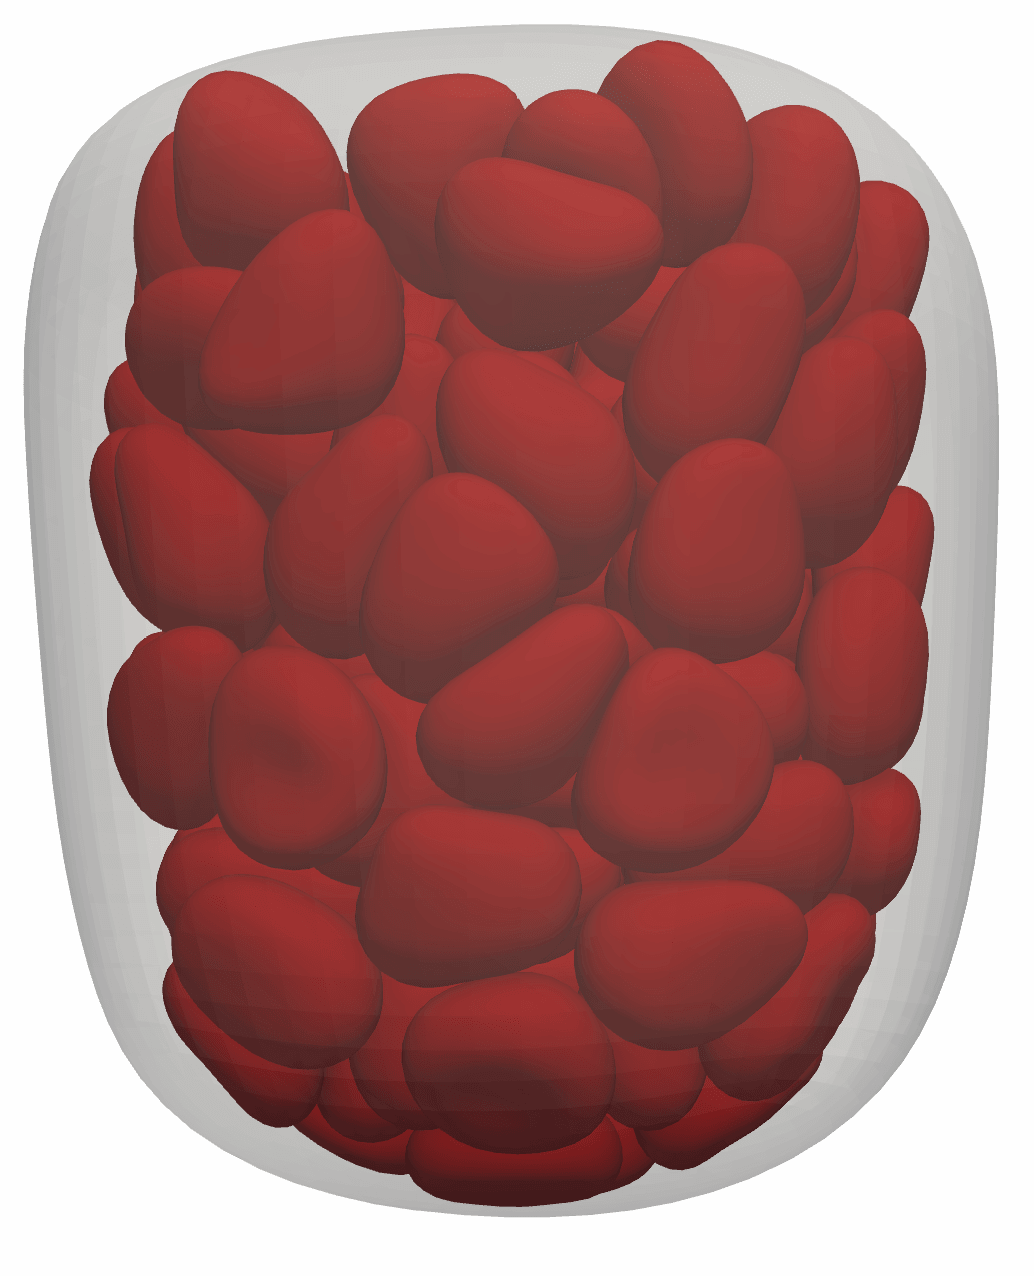
\includegraphics[angle=0,width=.98\linewidth]{high_vol_snap1}
\end{minipage}
\hspace{2ex}
\begin{minipage}[b]{0.2\textwidth}
    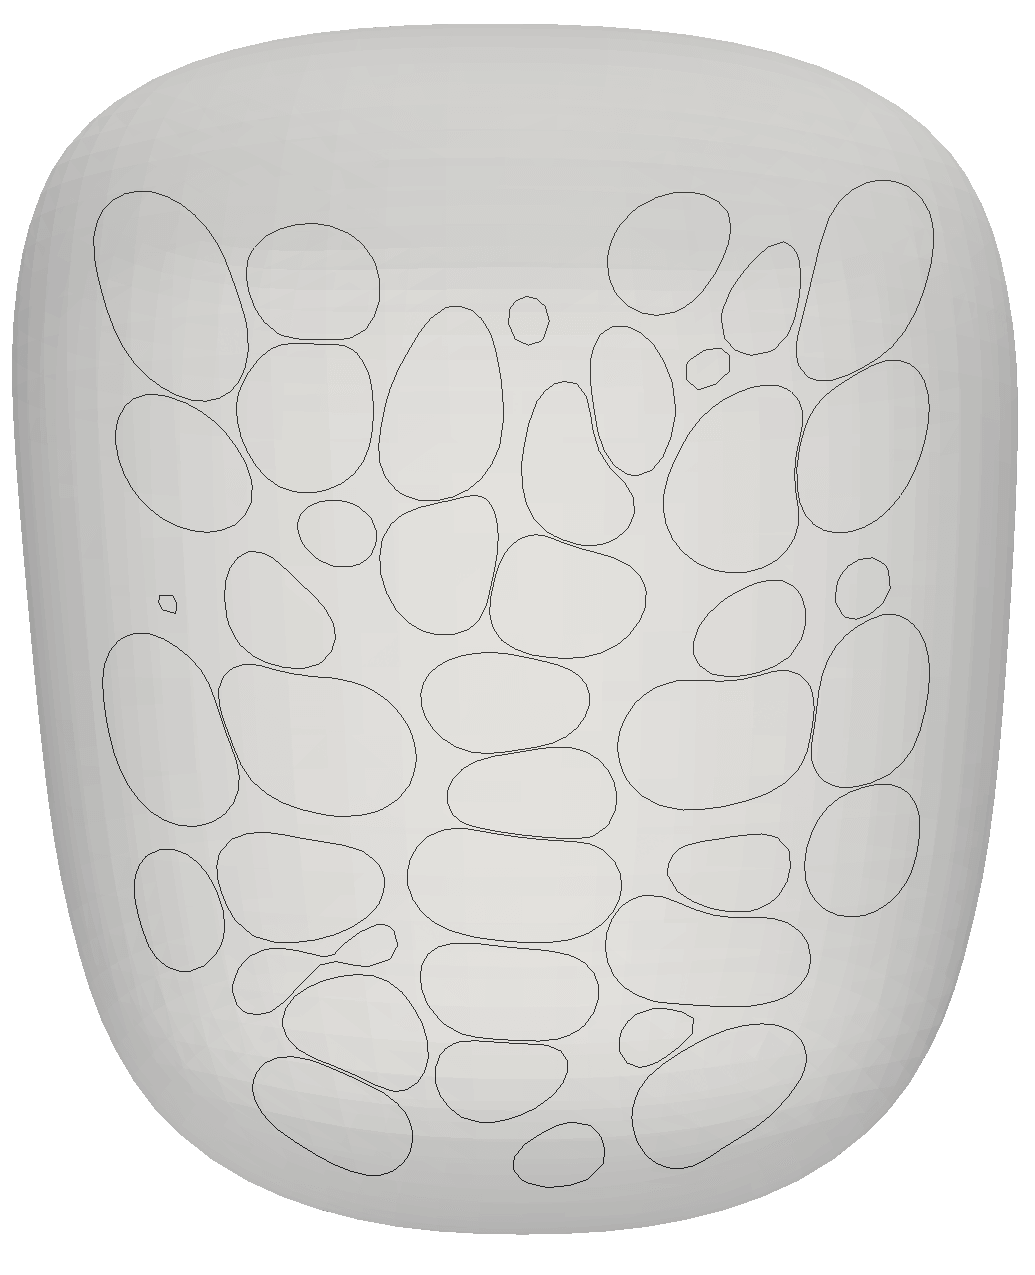
\includegraphics[angle=0,width=.98\linewidth]{high_vol_snap2}
\end{minipage}
\vfill
\begin{minipage}[b]{0.2\textwidth}
    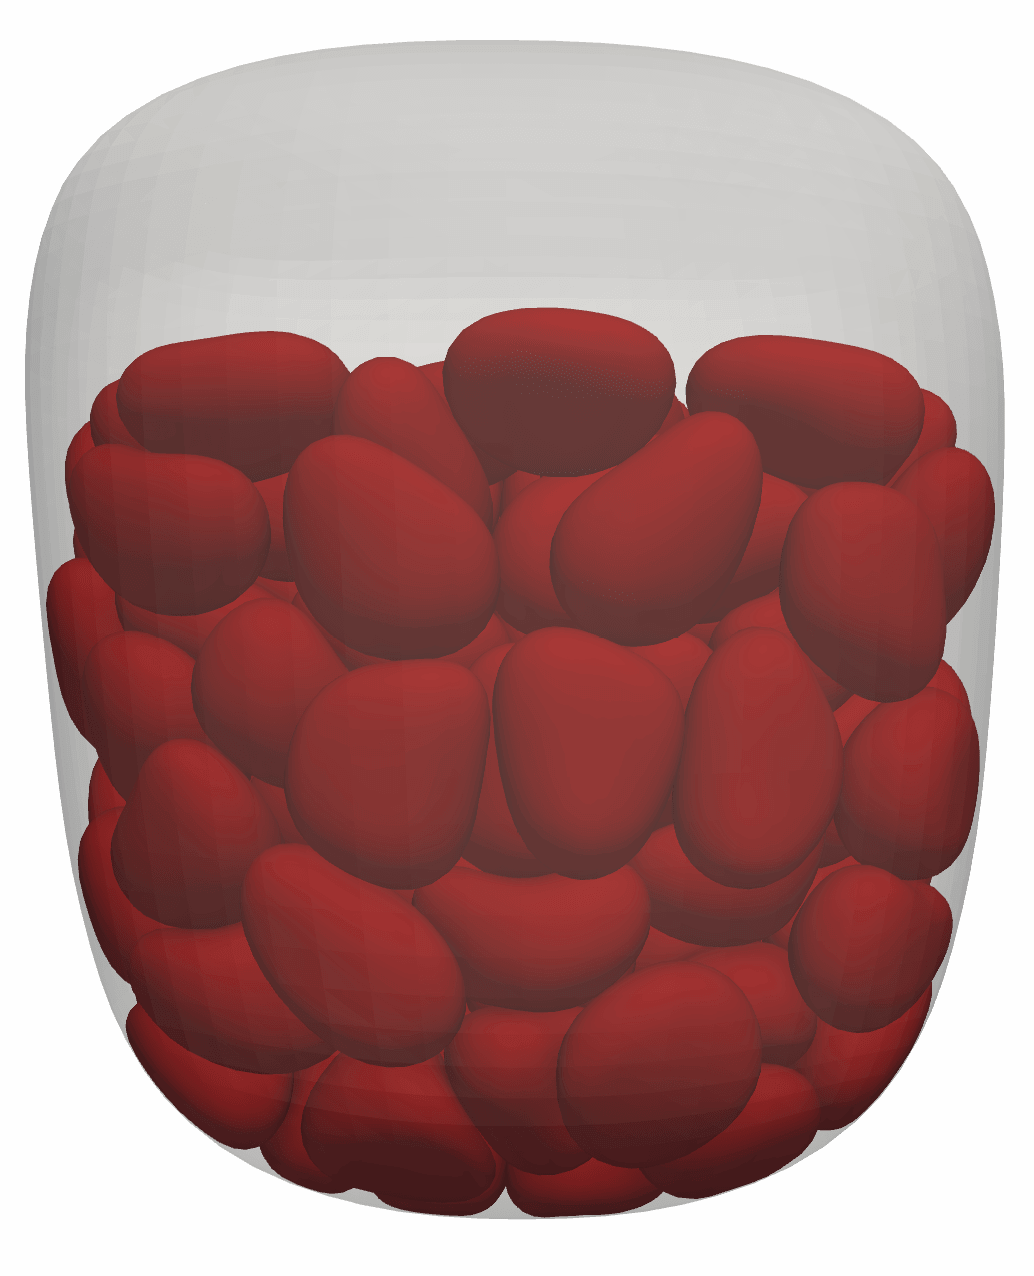
\includegraphics[angle=0,width=.98\linewidth]{high_vol_snap3}
\end{minipage}
\hspace{2ex}
\begin{minipage}[b]{0.2\textwidth}
    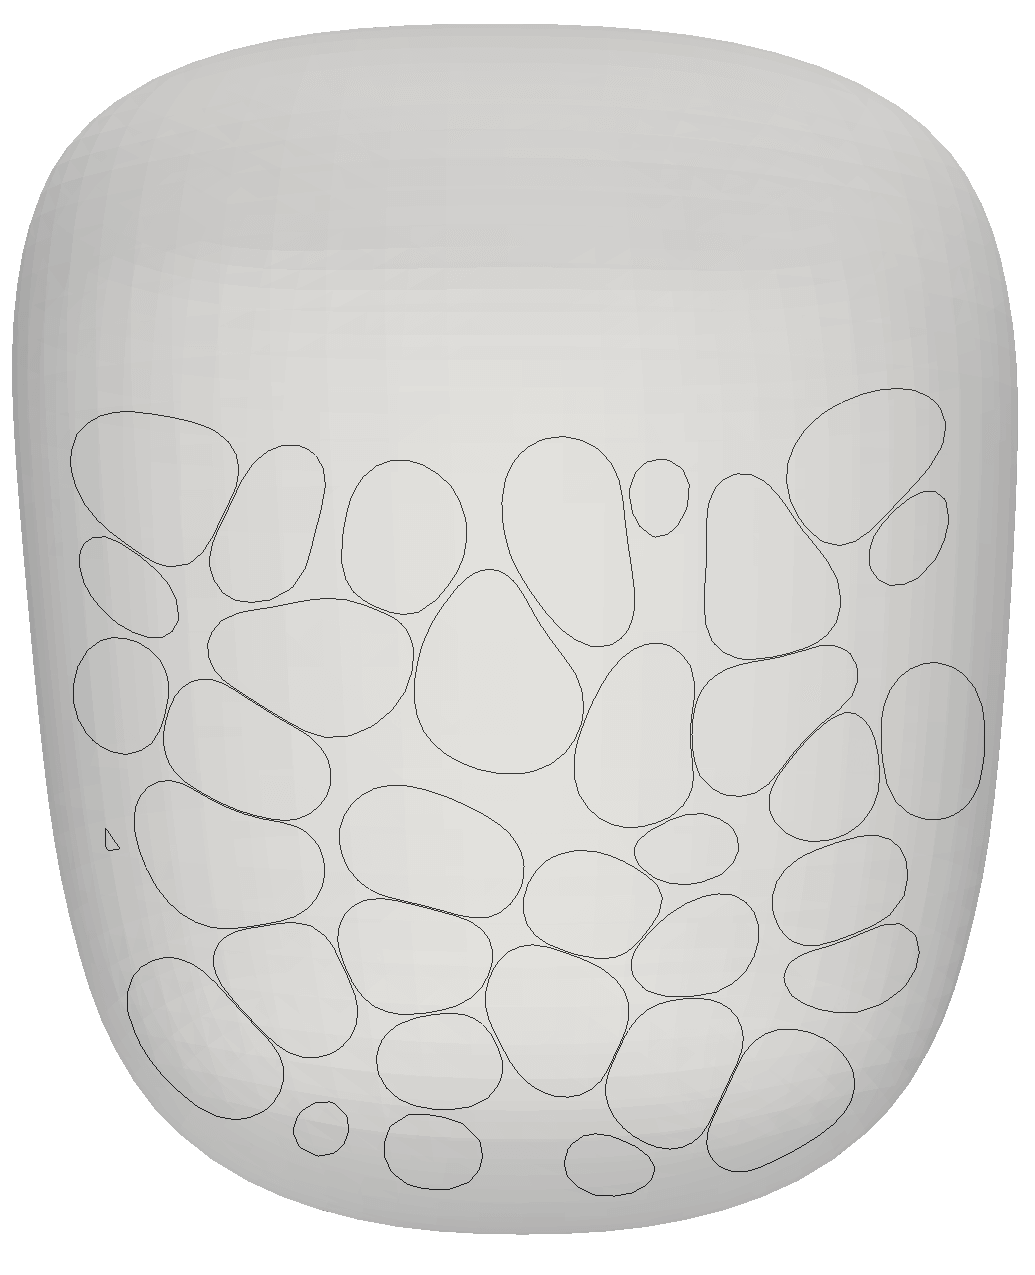
\includegraphics[angle=0,width=.98\linewidth]{high_vol_snap4}
\end{minipage}
    \mcaption{fig:high-vol-snap}{High-volume fraction
      sedimentation due to gravitational force.}{
    The initial configuration (top figures) has a volume fraction of $47\%$. 
    As the cells sediment to the lower part of the domain (bottom figures), the local
    volume fraction of the final state in this lower part of the
    domain is around $55\%$. Shown on the
    right side are slices through the center of the domain together
    with the \rbc boundaries in the initial and final configuration.
    The full simulation video is available at
    \href{https://vimeo.com/329509435}{\textcolor{blue}{https://vimeo.com/329509435}}.
}
\end{figure}
\textbf{Discretization and example setup. }
For all test cases we present, we discretize each \rbc with $544$ quadrature
points and 2,112 points for collision detection.
The blood vessel geometry is represented with 8th order tensor-product
polynomial patches with  121 quadrature points per patch and 484
equispaced points for collision detection.
The parameters chosen for singular/near-singular integration are $p=8$ and $\eta=1$, with $R=r=.15L$ for strong scaling tests and $R=r=.1L$ for weak scaling tests.
The value of $L$ is the square root of the surface area of the patch containing the closest point to the target, called the \emph{patch size}; this choice allows for a consistent extrapolation error over the entirety of $\Gamma$.

Since our scaling tests are performed on complex, realistic blood
vessel geometries, we must
algorithmically generate our initial simulation configuration.
We prescribe portions of the blood vessel as inflow and outflow regions and
appropriately prescribe positive and negative parabolic flows (inlet and outlet
flow) as boundary
conditions, such that the total fluid flux is zero.
To populate the blood vessel with \rbcs, we uniformly sample the volume of the 
bounding box of the vessel with a spacing $h$ to find point locations
inside the domain at which we place \rbcs in a random orientation.
We then slowly increase the size of each \rbc until it collides with the
vessel boundary or another \rbc; this determines a single \rbc's size.
We continue this process until all \rbcs stop expanding; this means that 
we are running a simulation of \rbcs of various sizes.
We refer to this process as \textit{filling the blood vessel with }\rbcs.
This typically produces \rbcs of radius $r$ with $r_0 < r < 2r_0$ with $r_0$ chosen proportional to $h$. 
This is a precomputation for our simulation, so we do not include this
step in the timings we report for weak and strong scaling.
We emphasize that these simulations are primarily for scaling purposes
of our algorithms and are not expected to represent true blood flows.
The platform can of course be applied to length scales where viscous
flow is a valid assumption.
%\note[MJM]{check}

Additionally, \rbcs in such a confined flow will collide with the
blood vessel wall
if special care is  not taken near the outflow part of the boundary.
We define regions near the inlet and outlet flows where we can safely add and
remove \rbcs.
When an \rbc $\gamma_i$ is within the outlet region, we subtract off the velocity due to
$\gamma_i$ from the entire system and move $\gamma_i$ into an inlet
region such that the arising \rbc
configuration is collision-free.

\textbf{Limiting \abbrev{GMRES} iterations. }
%We choose the complicated domains and \rbc configurations to present our
%algorithms' scalability on realistic simulation that are of practical interest.
%An downside of this decision is that the conditioning of double-layer
%integral operator in \cref{eq:double_layer_int_eq} is poorly conditioned due to
%the complex nature of the geometry.
We have observed that the GMRES solver typically requires 30 iterations
or less for convergence for almost all time steps, but the number
of needed iterations may vary more in the first steps. 
To simulate the amount of work in a typical simulation time
step, we cap the number of \gmres iterations at 30 and report weak and strong
scaling for these iterations. A more detailed analysis of this behavior is needed.

%This causes \gmres to stagnate without a good initial guess at the solution.
%As the simulation progresses and the fluid velocity becomes more smooth due to
%\rbc alignment, the density from the previous time step becomes a
%better initial guess, allowing \gmres reach the absolute tolerance in less than 30
%iterations. 
%\note[GS]{Should we say that we'll
%  figure out why this is and rerun for the final paper?}


\begin{figure*}[!bht]
\centering
  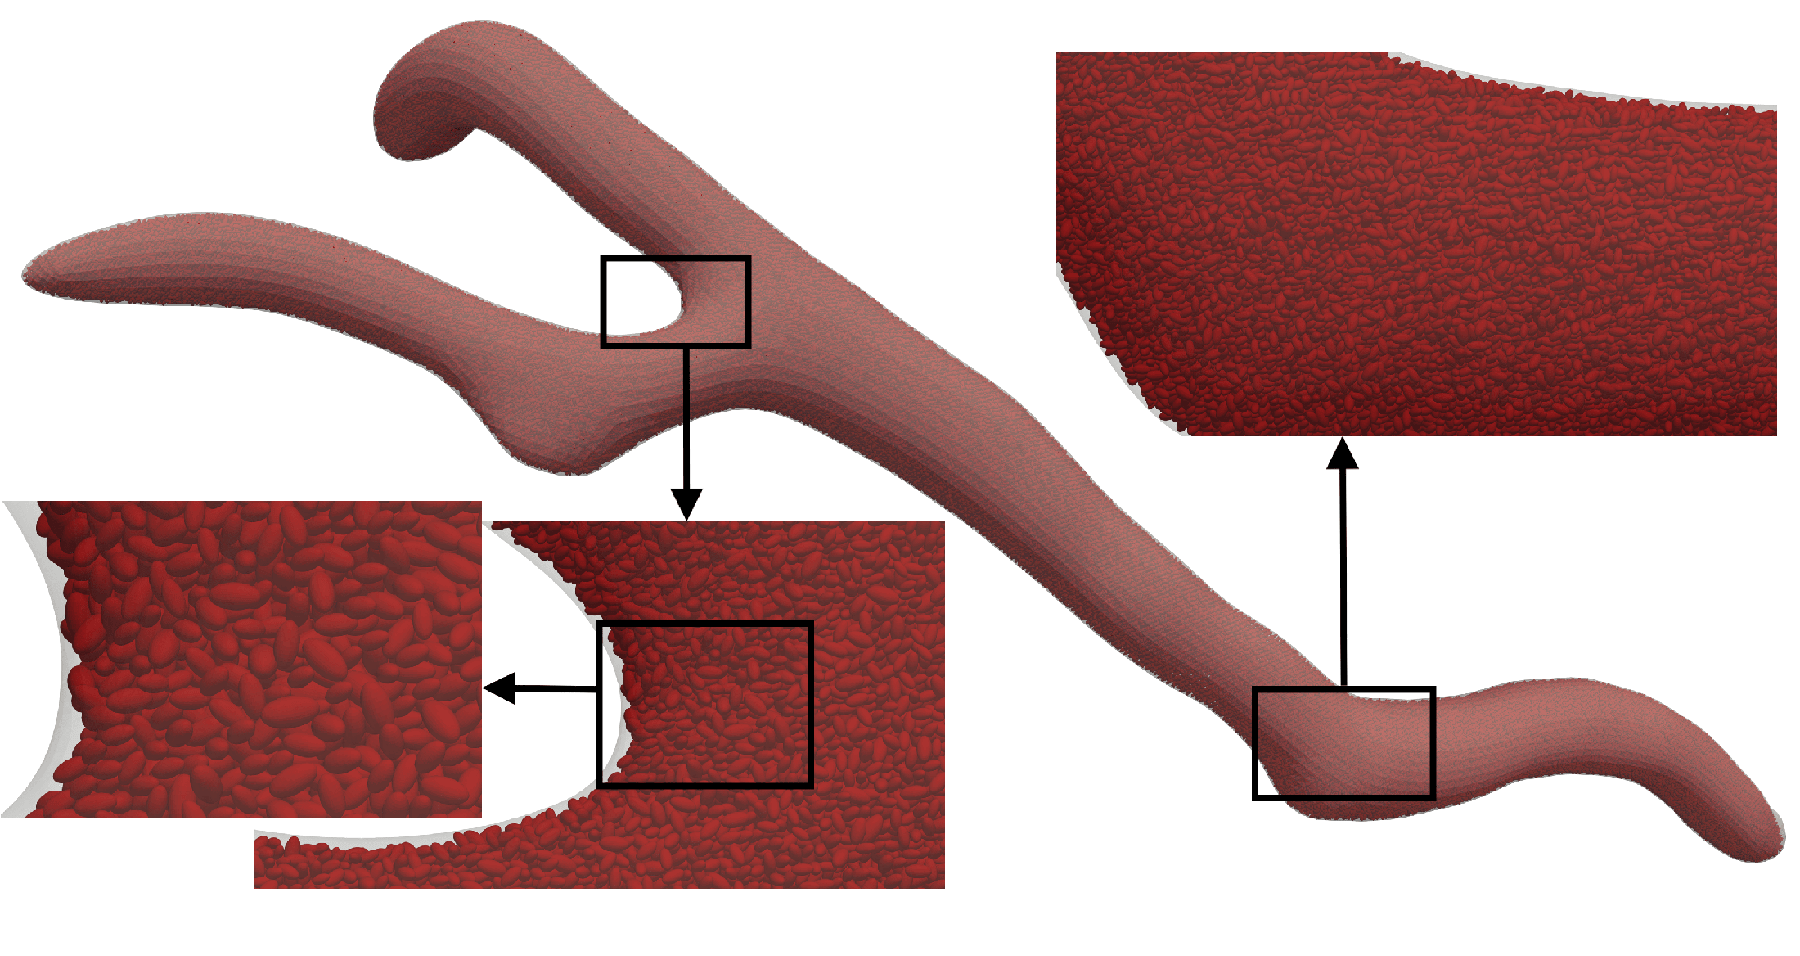
\includegraphics[angle=0,width=.85\linewidth]{weak_snap1}
  \mcaption{fig:wsscale-domain}{Weak scaling vessel geometry}{
    For our weak scaling experiments, we use the the vessel geometry
    shown above with inflow boundary conditions on the
    right side and outflow boundary condition on the two left sides.
    %\note[GS]{Matt/Libin, is that correct?}\note[LL]{correct}. 
    To setup the problem, we fill the vessel with 
    nearly-touching \rbcs of different sizes to obtain a desired
    number, and refine the
    vessel geometry patches. The figure above shows a setup with overall
    262,144 \rbcs at a volume fraction of $26\%$. 
  }
\end{figure*}


\subsection{Parallel scalability}\label{ss:scalability}

  Here, we present strong and weak scalability results for our \rbc simulations. 
  We decompose the time required for a complete simulation into the following categories:%\note[MJM]{fix vspace}
 \begin{itemize}
    \item {\bf\em COL}: detection and resolution of collisions among
      \rbcs and between \rbcs and the vessel walls;
      \item {\bf\em BIE-solve}: computing $\vu^{\Gamma}$, not including \fmm calls. This includes all of the steps for singular/near-singular integration in \cref{sec:solver} except the evaluation $\vu^\Gamma$ at the check points.
      \item {\bf\em BIE-FMM}: \fmm calls required to evaluate $\vu^{\Gamma}$ at the check points and at points on \rbcs
      \item {\bf\em Other-FMM}: \fmm calls required by other algorithms 
      \item {\bf\em Other}: all other operations
  \end{itemize}
In the discussion below, we focus on {\bf\em COL} and {\bf\em BIE-solve}, as
  they are the primary algorithmic contribution of this work, and discuss
  how to reduce the computational time required for {\bf\em BIE-FMM}.

\textbf{Strong scalability. }\label{ss:strong}
To study the strong scalability of our algorithms, we use the blood vessel
geometry and \rbc configuration in
\cref{fig:strong-scale-domain}-left.
This simulation contains 40,960 \rbcs and the blood vessel is
represented with 40,960 patches.
%we discretize each \rbc with $544$ quadrature
%points and 2,112 points for collision detection.
%\rbc dofs = 89,128,960, boundary dofs = 14,868,480
With four degrees of freedom per \rbc quadrature point and three per vessel
quadrature point, this amounts to
89,128,960 and 14,868,480 degrees for the \rbcs and blood vessel, respectively 
(103,997,440 in total).
%We report the wall-time for $10$ time steps in \cref{fig:sscale}, 
As can be seen from \cref{fig:sscale}, we achieve a $15.7$-fold
speed-up in total wall-time scaling from 384 to 12288 cores,
corresponding to $49\%$ parallel efficiency.  This level of  parallel
efficiency is partially due to the calls to the fmm library
\pvfmm. The strong scalability of \pvfmm we observe is largely
consistent with the results reported in \cite{malhotra2016algorithm}.
Neglecting the time for calls to \fmm, i.e., only counting the time
for the boundary solver to compute $\vu^\Gamma$ and for collision
prevention, we find $66$\%
parallel efficiency when scaling strongly from 384 to 12288 cores.
We see that the parallel collision handling and integral equation solver
computations, excluding \fmm, scale well as the number of cores is increased.

\textbf{Weak Scalability. }\label{ss:weak}
Our weak scalability results are shown in
\cref{fig:wscale-large-grain,fig:wscale-knl}.
Both tests are performed on the blood vessel displayed in
\cref{fig:wsscale-domain}.
We use an initial boundary composed of a fixed number $M$ of polynomial
patches and fill the domain with roughly $M/2$ \rbcs (which requires spacing
$h$).
To scale up our simulation by a factor of four, we: (1) subdivide the $M$ polynomial
patches into $4M$ new but equivalent polynomial patches (via subdivision rules
for Bezier curves); (2) refill the domain with \rbcs using spacing 
$h/\sqrt[3]{4}$. This places $2M$ \rbcs in the domain volume.
We repeat this process each time we increase the number of cores by a factor of
four in order to keep the number of patches and \rbcs per core constant.
In the tables in  \cref{fig:wscale-large-grain,fig:wscale-knl},
we report parallel efficiency with respect to the
first multi-node run on both \skx and \knl architectures, i.e, with
respect to 192 and 136 cores, respectively.
%\note[MJM-GS]{think that's ok now}

The largest weak scaling test contains 1,048,576 \rbcs and 2,097,152 polynomial
patches on the blood vessel; we solve for 3,042,967,552 unknowns at each time
step and are able to maintain a collision-free state between
4,194,304,000 triangular surface elements at each time step.
Comparing the weak scalability results for \abbrev{SKX}
(\cref{fig:wscale-large-grain}) and \abbrev{KNL}
(\cref{fig:wscale-knl}), we observe similar qualitative
behavior. Note that the smallest test on the \abbrev{SKX} architecture
only uses a single node, i.e., no MPI communication was needed. This
explains the increased time for the collision prevention algorithms when going
from 1 (48 cores) to 4 nodes (192 cores). 
Note also that the simulation on the \abbrev{KNL} architecture
used a significantly lower number of \rbcs and geometry patches per
node. Thus, this simulation has a larger ratio of communication to
local work. This explains the less perfect scalability compared to
the results obtained on the \abbrev{SKX} architecture.
As with strong scaling, we see good parallel scaling of the non-\fmm-related parts
of the computation of $\vu^\Gamma$ and the collision handling algorithm.

Note that there is a slight variation in the number of collisions for
the run on 8704 cores on \knl.
This is an artifact of the \rbc filling algorithm.
Since we place \rbcs in random orientations and distribute \rbcs
randomly among processors, we do not have complete control over the percentage
of collisions or the volume fraction for each simulation in
\cref{fig:wscale-large-grain,fig:wscale-knl}, as can be seen from
the tables under these figures.
This can affect the overall scaling: For the run on 8704 cores, the
percentage of collisions is larger, explaining the longer
time spent in {\bf\em COL}.
Despite this phenomenon, we achieve good weak scaling overall.
%This could be addressed by constructing a simpler weak scaling example, but at the expense of physical relevance of the simulation.
%\note[MJM]{possibly cut} %due to new run this paragraph might not be needed
%For collisions, vesicles are randomly distributed so are collisions, the load
%balance may cause the variance. 
%Also tests on KNL also has smaller grain size(per node) than tests on SKX.
%In general, we observe better performance/scaling on SKX nodes than KNL nodes.

\textbf{Discussion. }
The parts of the algorithm introduced in this paper scale as well as
or better than the \fmm implementation we are using.  However, our
overall run time is diminished by the multiple expensive
\fmm evaluations required for solving \cref{eq:double_layer_int_eq}.
This can be addressed by using a \textit{local} singular quadrature scheme,
i.e., compute a singular integral using the \fmm on
\cref{eq:smooth_double_layer_int_eq_patches_disc} directly, then compute a
singular correction locally.
This calculation has a three-fold impact on parallel scalability: (1) the \fmm
evaluation required is proportional to the size of the coarse discretization
rather than the fine discretization ($O((p+1)N)$ vs.\ $O((k+p)N)$);
(2) after the \fmm evaluation, the local correction is embarrassingly parallel;
(3) the linear operator \cref{eq:sing-quad} can be precomputed, making the
entire calculation extremely fast with \abbrev{MKL} linear algebra routines.
These improvements together will allow our algorithm to scale well beyond the
computational regime explored in this work.

\subsection{Verification}
There are few analytic results known about \rbcs in confined Stokes
flows against which we can verify our simulations. However,
exact solutions can be obtained for a part of our setup, invariants
(e.g., surface area) can be considered and solutions for smaller examples can
be verified against solutions with fine spatial and temporal discretizations.
In particular, in this section, we demonstrate the accuracy of the parallel boundary
solver presented in \cref{sec:solver} and numerically study the collision-free
time-stepping in \cref{sec:parallel-contact}. 
%The other components of our overall method, referred to in \cref{sec:alg_overview}, are also known to be highly accurate.

\textbf{Boundary solver. }
The error of the boundary integral solver is determined
by the error of integration and the GMRES error, the latter not depending on the number of discretization points due to good conditioning of the equation.  The integration error, in turn, can be separated into smooth quadrature error and interpolation error. The former is  high-order accurate \cite{trefethen2013approximation}.
Although our extrapolation is ill-conditioned, we observe good accuracy for $p\leq 8$. The singular evaluation in \cref{sec:solver} converges with rate
$O(L^p + L^q)$ corresponding to $p$th order extrapolation and $q$th
order quadrature.
To confirm this numerically, we solve an interior Stokes problem on the
surface in \cref{fig:boundary-err}-right.
We evaluate a prescribed analytic solution at the discretization
points to obtain the boundary condition.
We then solve \cref{eq:int_eq_disc} and compare the numerical
solution at on-surface samples different from discretization points, evaluated using the algorithms of \cref{sec:solver}. 
We use $\eta =2$, $q=16$, $p=8$, $R=.04\sqrt{L}$ and $r = R/8$.
In \cref{fig:boundary-err}-left, we report the relative error in the
infinity-norm of the velocity.
By choosing check point distances proportional to $\sqrt{L}$,
%we observe the expected convergence as described in \cite{klockner2013quadrature}, and
we observe the expected $O(L^7)$ convergence.
%\note[GS]{I dont think I fully understand that convergence test.}
%We see that the extrapolation error is dominant and observe the expected $O(L^7)$ convergence
\begin{figure}[h]
  \centering
%\begin{minipage}[b]{.2\textwidth}
\begin{tikzpicture}
  %
  \begin{loglogaxis}[%
    width=2.62in,
    height=1.875in,
      scale only axis,
      separate axis lines,
      every outer x axis line/.append style={white!15!black},
      every x tick label/.append style={font=\color{white!15!black}},
      %xmin=100,
      %xmax=10000,
      xlabel={Max patch size},
      every outer y axis line/.append style={white!15!black},
      every y tick label/.append style={font=\color{white!15!black}},
      %ymin=5e-2,
      %ymax=1,
      ylabel={Max relative error},
      ytick={1e-1,1e-3,1e-5, 1e-7, 1e-9},
      xlabel style={font=\small},
      ylabel style={font=\small},
      legend pos=north west,
      legend cell align=left,
    ]

    \addplot [color=plt-orange,line width=1.0pt,mark=square*,mark size=1.2pt,mark repeat=1,mark phase=0]
        table[x index=0,y index=1]{figs/bie-conv.dat};
    %    \addlegendentry{$\max_i\|\vu_i-\hat{vu}_i\|_\infty/\|\vu_i\|_\infty$}
        \addlegendentry{Max rel. error}

    \addplot [color=black,line width=1.0pt,dotted,domain=5e-2:.4]{400*x^7};
    \addlegendentry{$O(L^7)$}
  \end{loglogaxis}
\end{tikzpicture}
%\end{minipage}
%\hspace*{.1\linewidth}
%\begin{minipage}[b]{0.2\textwidth}
%\begin{minipage}[b]{0.25\textwidth}
    %\hspace*{-.05\linewidth}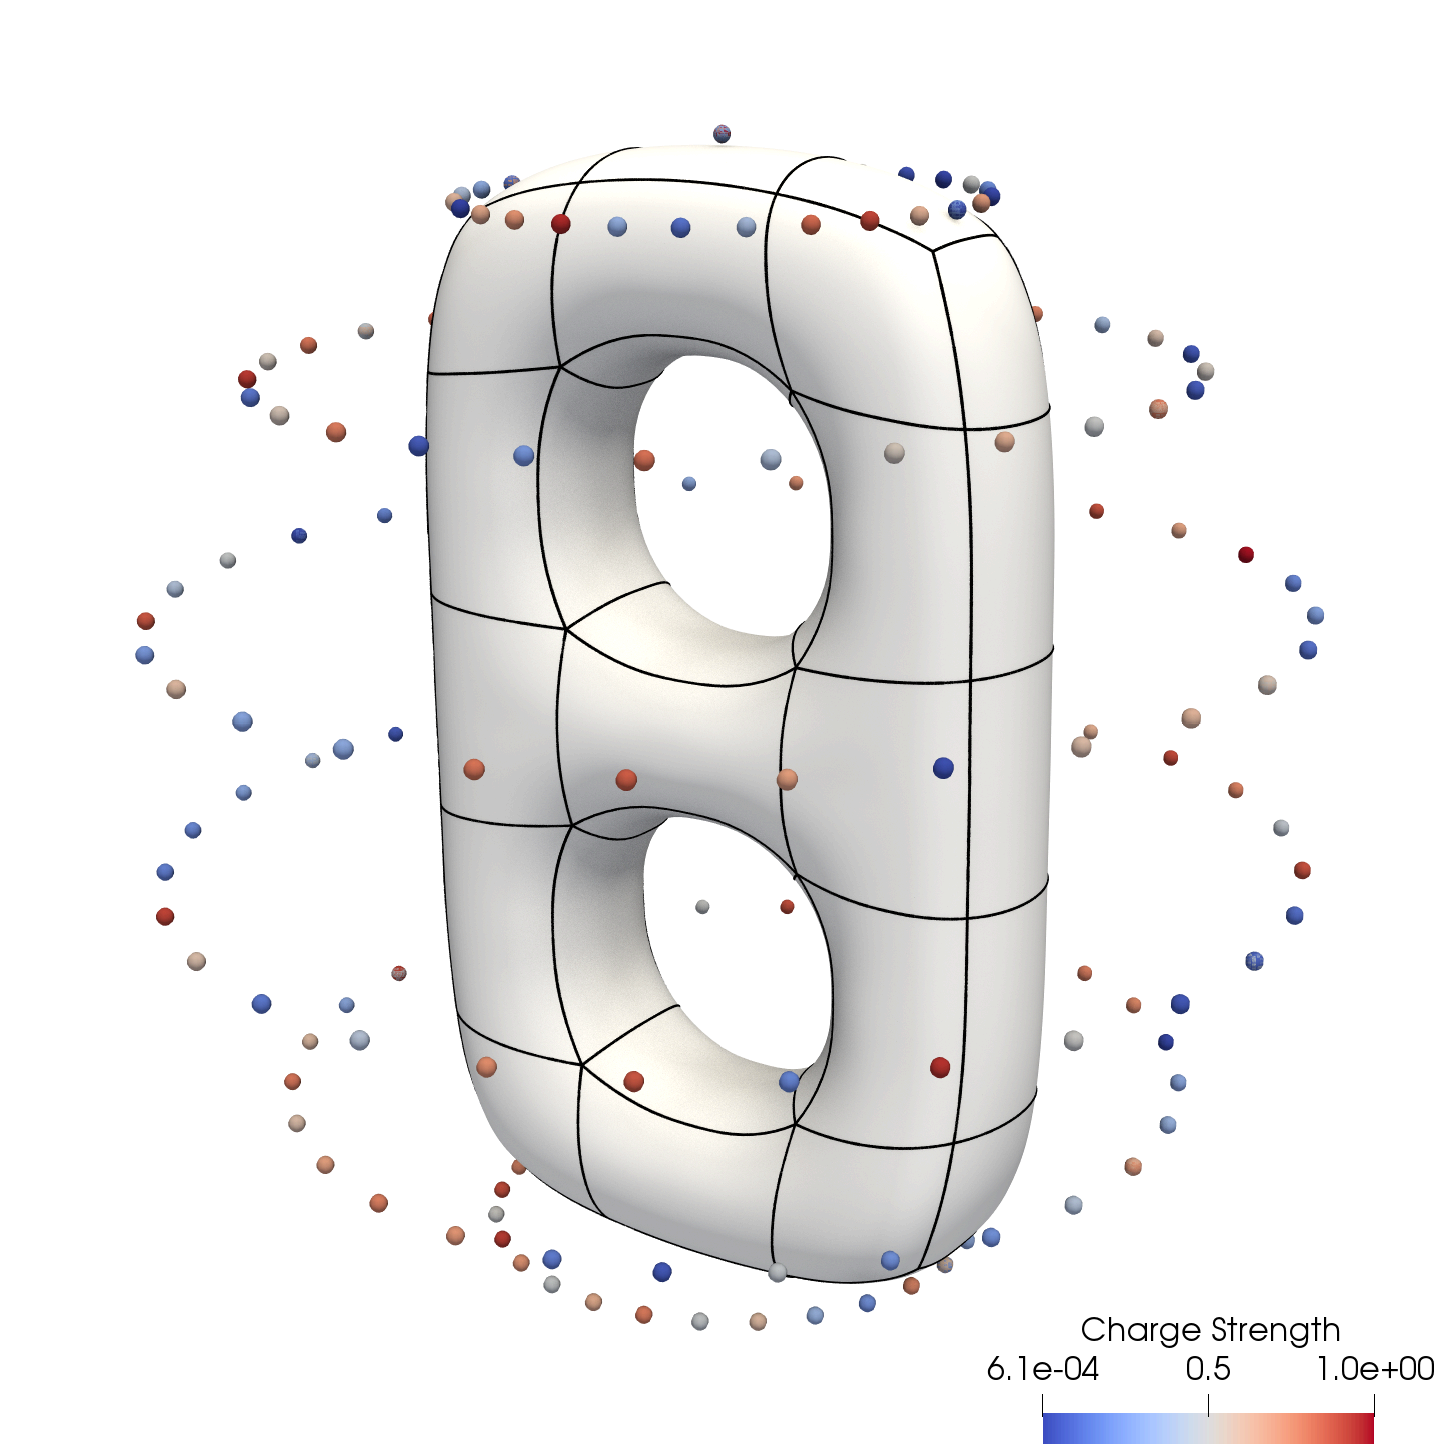
\includegraphics[angle=0,width=.3\linewidth]{figs/ttorus2_convergence_setup.png}
%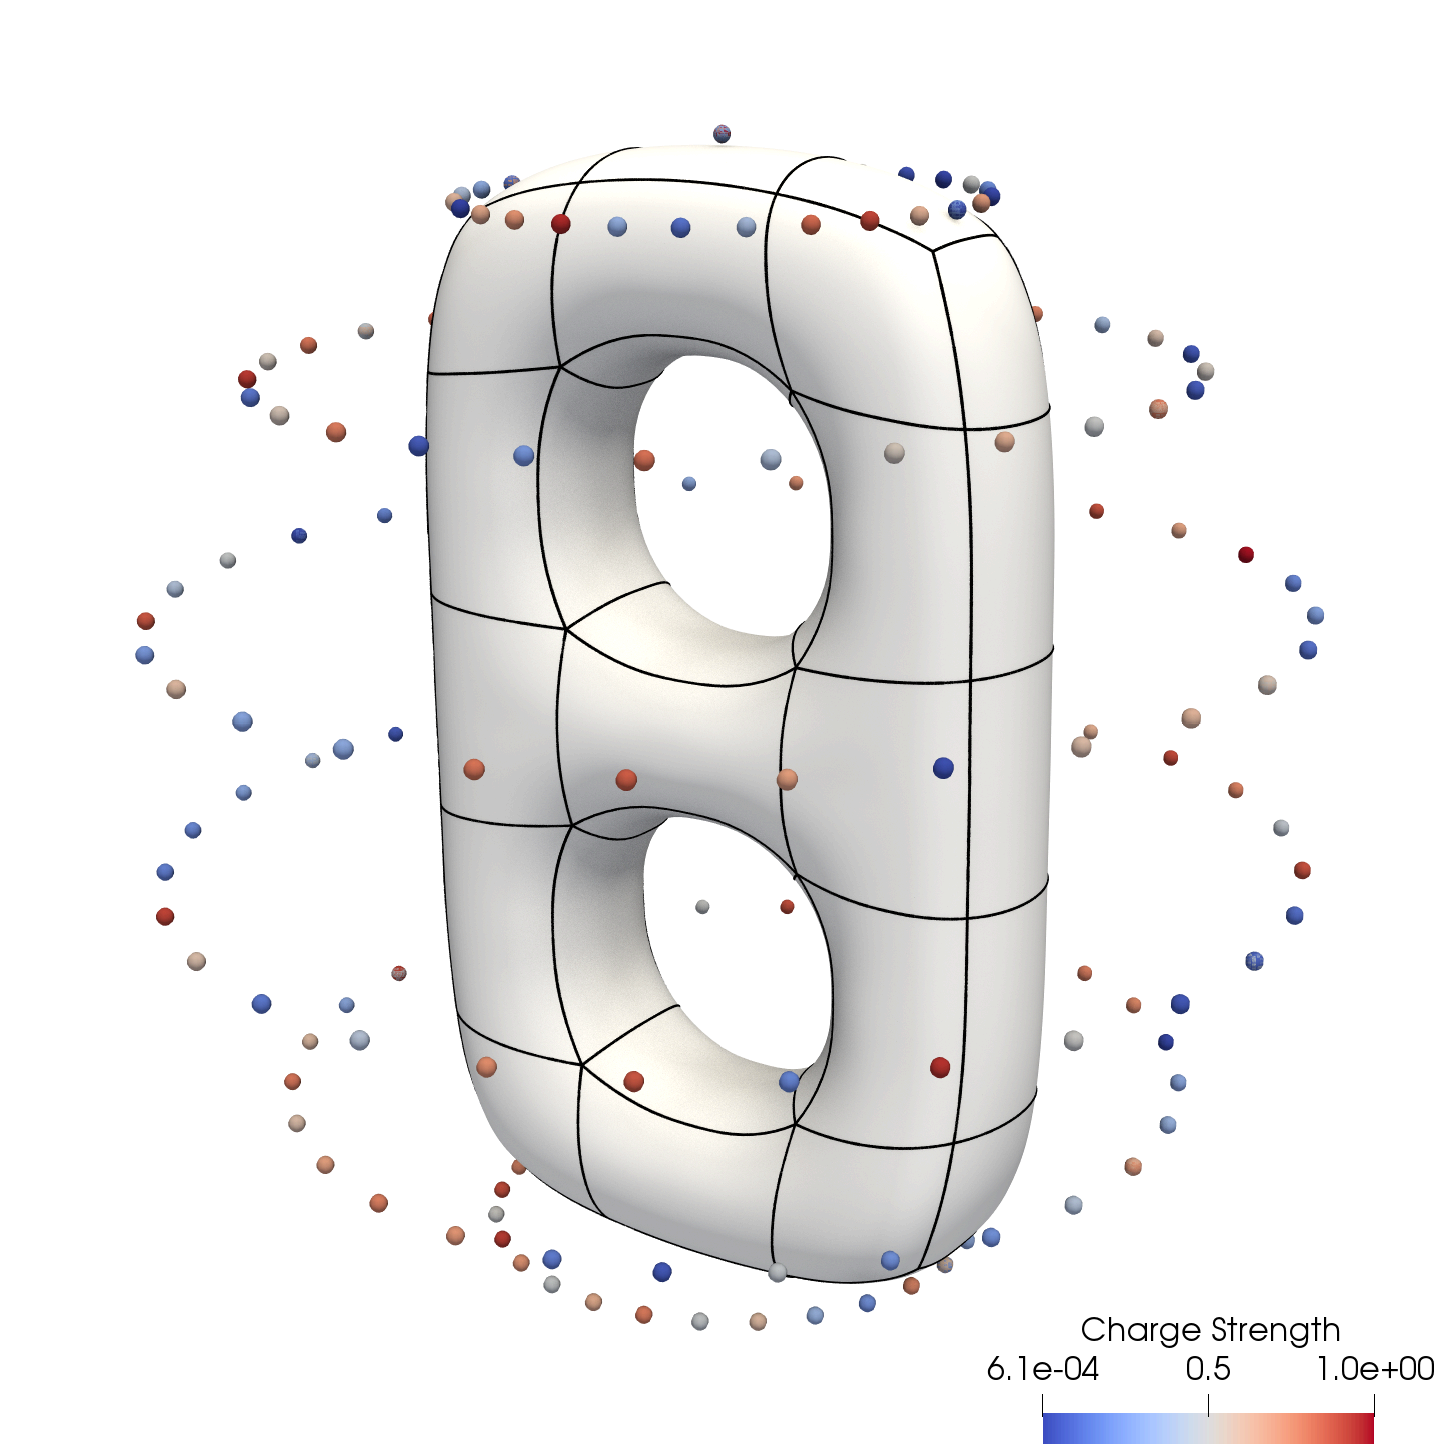
\includegraphics[angle=0,width=\linewidth]{figs/ttorus2_convergence_setup.png}
%\end{minipage}%
\mcaption{fig:boundary-err}{
    Error convergence test solving \cref{eq:int_eq_disc} with \qbkix on the domain \cref{fig:solver-conv-test-cases}-right .}{
  We evaluate a known solution on the coarse discretization and solve for $\phi$.
On the left, we plot the maximum relative error in the infinity norm
of $\vu^\Gamma$ evaluated on the surface. 
On the right, we show the coarse discretization of the domain boundary
and patches.
%in the coarse discretization of \cref{eq:int_eq_disc}.
}  %\vspace{-5pt}
%\end{minipage}
\end{figure}

\textbf{\rbcs with collision resolution and convergence. }
Our choice of \rbc  representation and discretization is spectrally
accurate in space for the approximation, differentiation and
integration of functions on \rbc  surfaces, as shown in
\cite{Veerapaneni2011}. Although we use first-order time-stepping in
this work,   \emph{spectral deferred correction} (\abbrev{SDC}) can be
incorporated into the algorithm exactly as in the 2D version described
in  \cite{lu2017}. This present work demonstrates second-order convergence in
time; however, \abbrev{SDC} can be made arbitrarily high-order
accurate.

For collision-resolution accuracy verification, we study the
convergence of our contact-free time-stepping with two \rbcs in shear
flow. As shown in \cref{fig:shear-snap}, at $T=0$, two \rbcs are
placed in a
shear flow $\vu = [z,0,0]$ in free-space. % with a vertical offset $\delta_0=0$.
We first compute a reference solution without
collision handling  but with expensive adaptive fully implicit time-stepping to
ensure accurate resolution of the lubrication
layer between \rbcs. This reference simulatation used spherical
harmonics of order 32 and the time step had to be reduced to
6.5e-4 to prevent collisions.
In \cref{fig:shear-conv}, we show the convergence for the error in the centers of mass of each \rbc as a function of the time-step size. 
We use spherical harmonic orders $16$ and $32$ for the spatial
discretization to demonstrate the dominance of the time-stepping error. 
We observe first-order convergence with our locally-implicit backward Euler scheme which confirms that our collision resolution algorithm does not have a significant impact on time-stepping accuracy.
%87, 58
\todo{add back in vesicle validation fig}
\begin{figure}[!htb]
  \centering
  \hfill
  \begin{minipage}{.25\textwidth}
      \centering
    %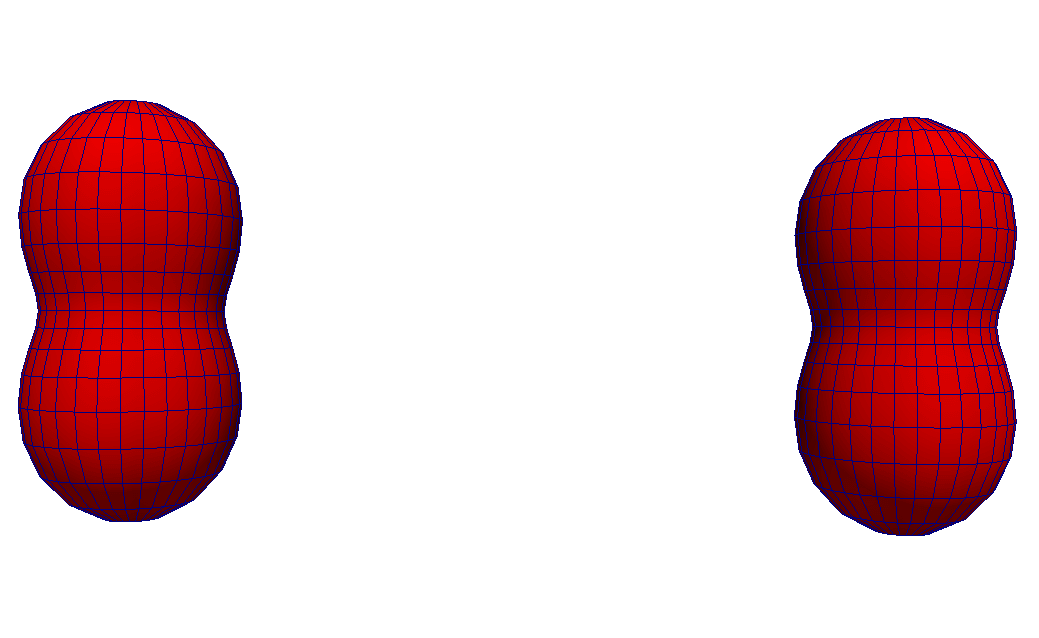
\includegraphics[width=52pt,height=35pt]{shear1}
    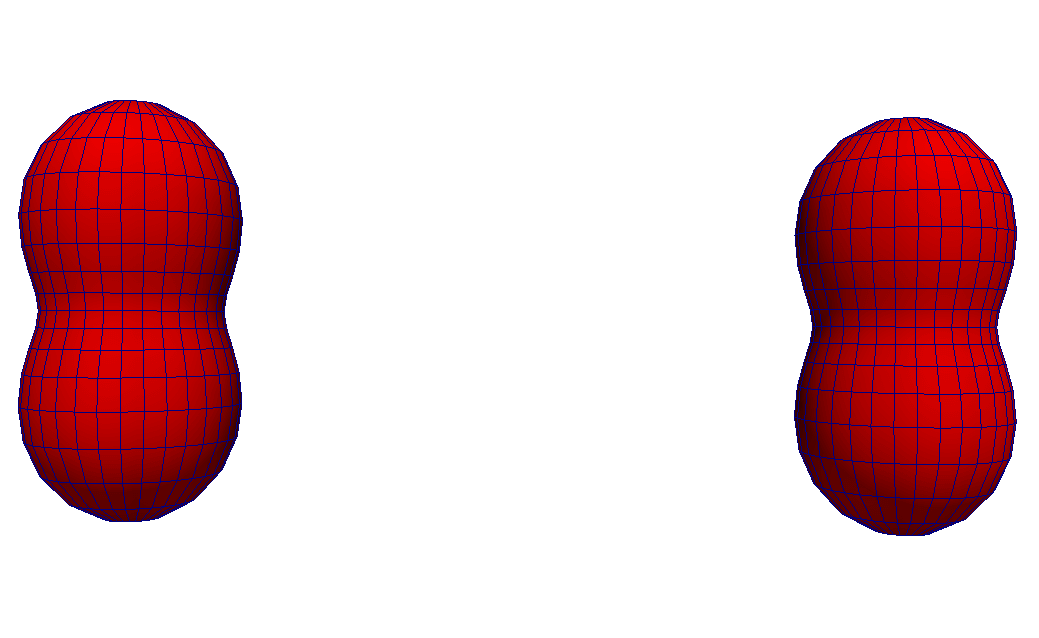
\includegraphics[width=.95\linewidth]{shear1}
  \end{minipage}\hfill
  \begin{minipage}{.25\textwidth}
      \centering
    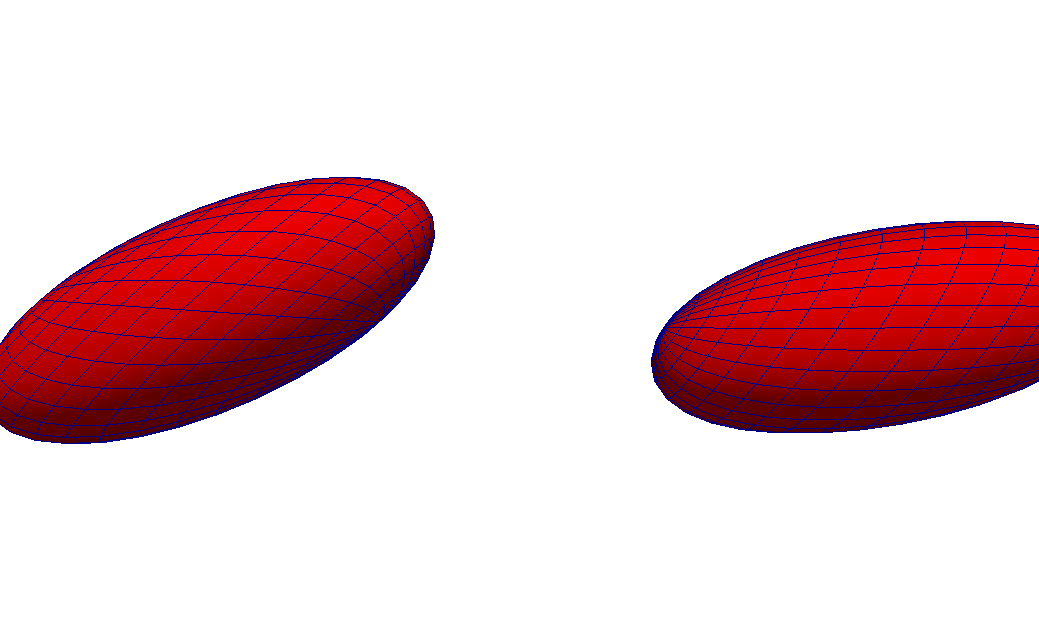
\includegraphics[width=.95\linewidth]{shear2}
  \end{minipage}\hfill
  \begin{minipage}{.25\textwidth}
      \centering
    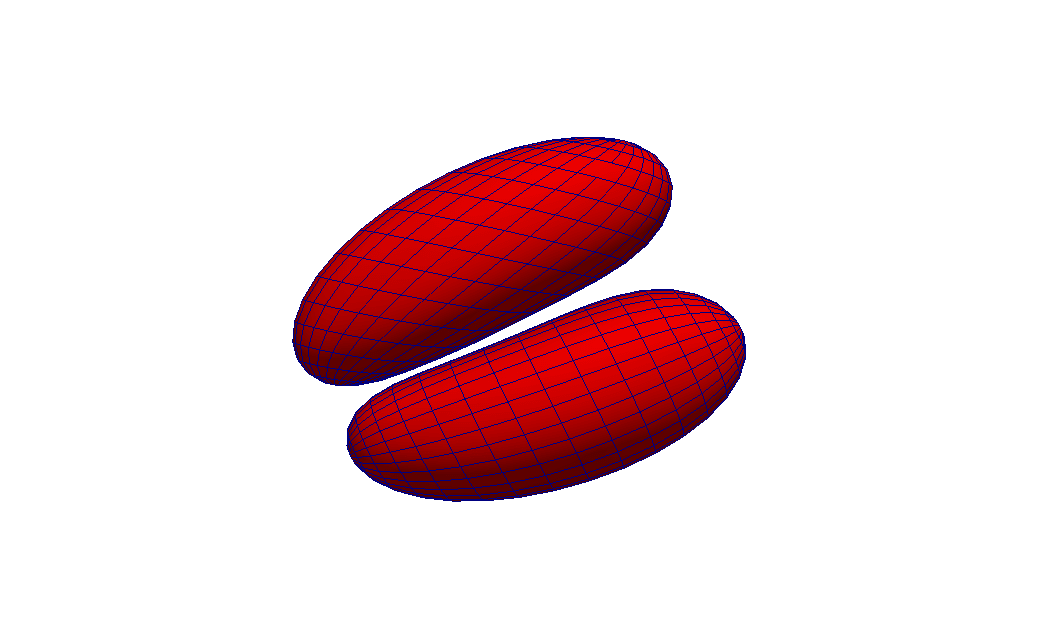
\includegraphics[width=.95\linewidth]{shear3}
  \end{minipage}\hfill
  \begin{minipage}{.25\textwidth}
      \centering
    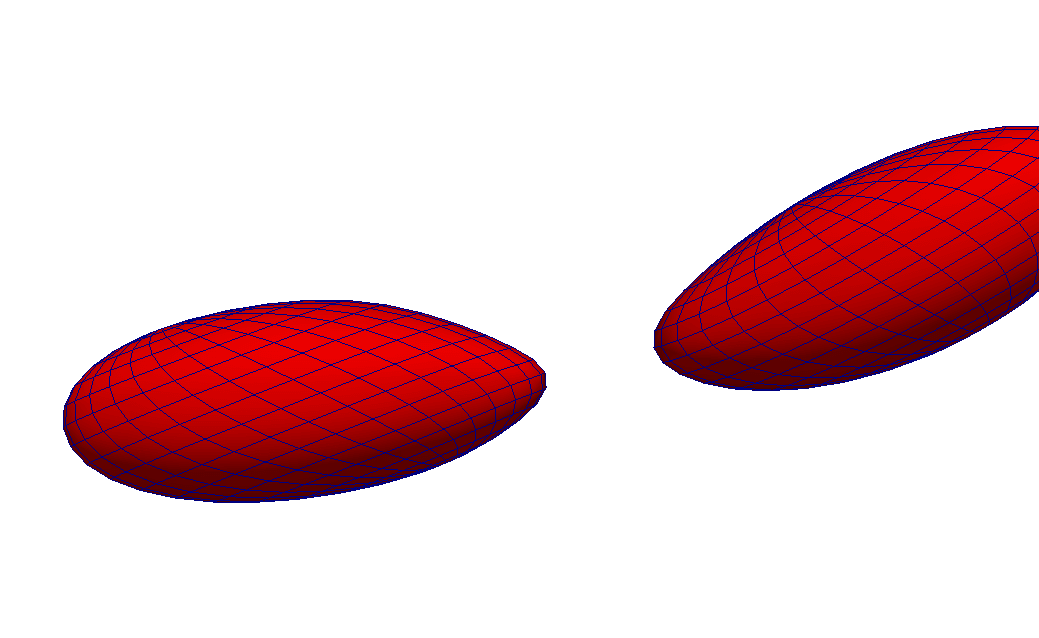
\includegraphics[width=.95\linewidth]{shear5}
  \end{minipage}\hfill
    \mcaption{fig:shear-snap}{Snapshots of two vesicles in shear flow}{ %\vspace{-5pt}
    At $T=0$, two vesicles are placed at $[-5.5, 0, 0]$ and $[0, 0, 0]$ respectively.}
\end{figure}%

%\begin{figure}[!htb]
%  \subfloat[$t=0$\label{sfg:shear-snap1}]{\framebox(52,35){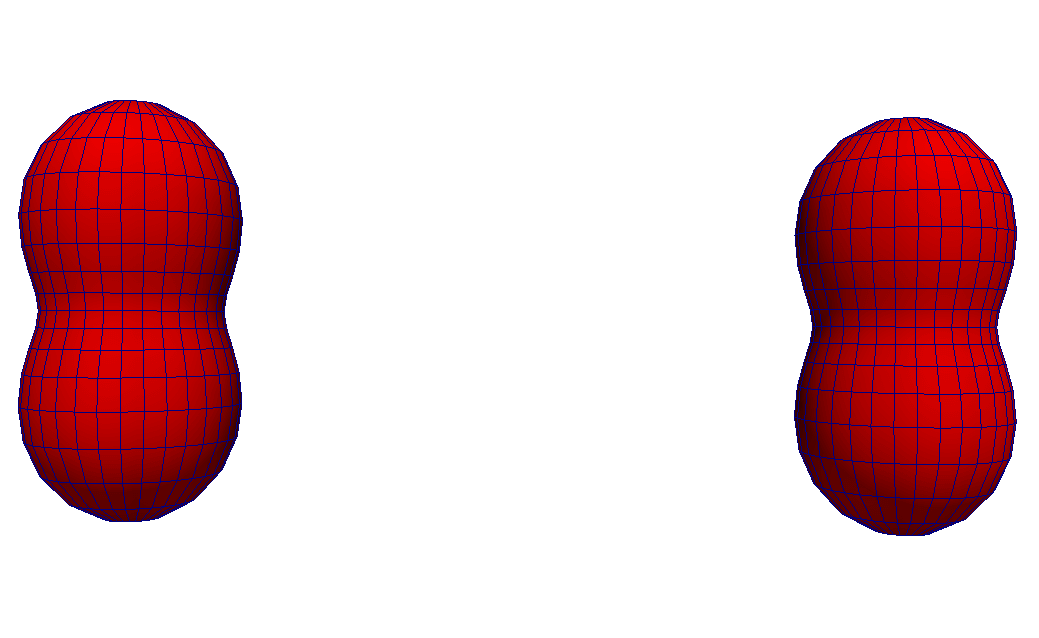
\includegraphics[width=52pt,height=35pt]{shear1}}}
%  \hspace{1pt}
%  \subfloat[$t=5$\label{sfg:shear-snap2}]{\framebox(52,35){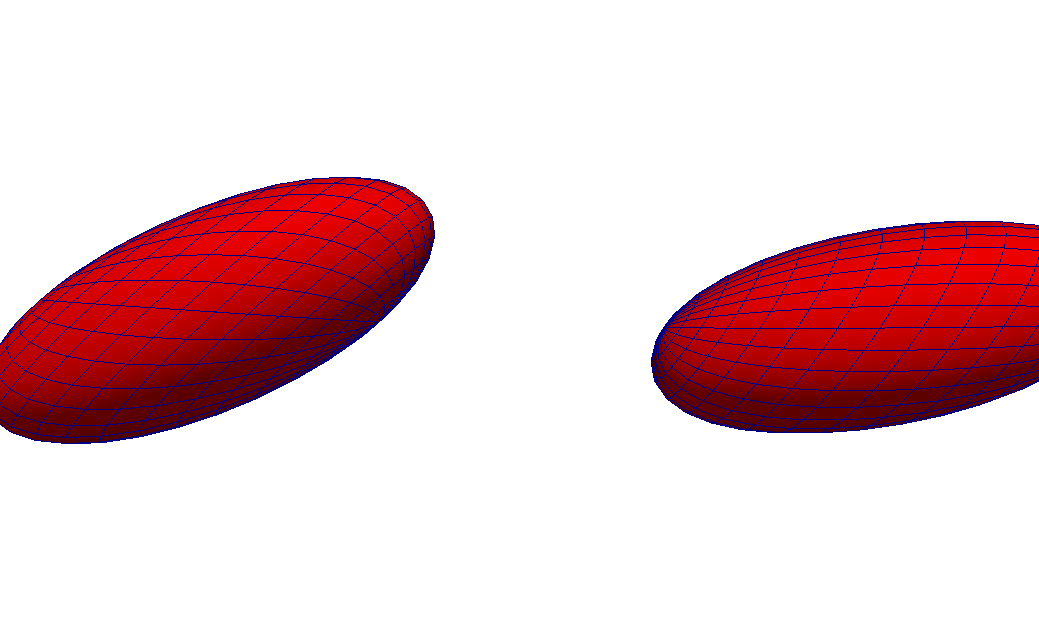
\includegraphics[width=52pt,height=35pt]{shear2}}}
%  \hspace{1pt}
%  \subfloat[$t=20$\label{sfg:shear-snap3}]{\framebox(52,35){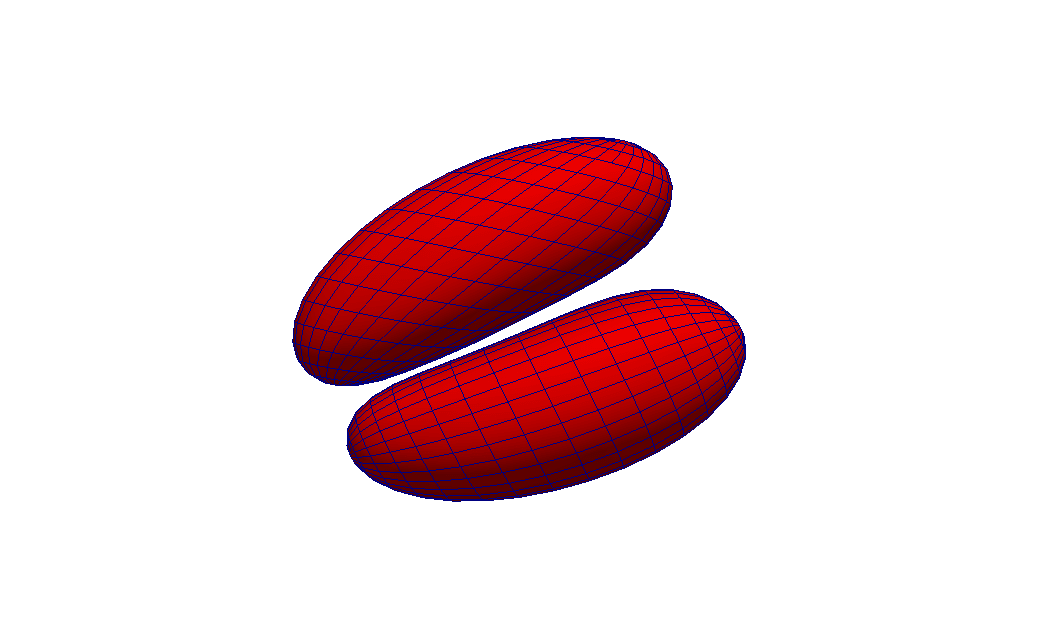
\includegraphics[width=52pt,height=35pt]{shear3}}}
%  \hspace{1pt}
%  \subfloat[$t=25$\label{sfg:shear-snap4}]{\framebox(52,35){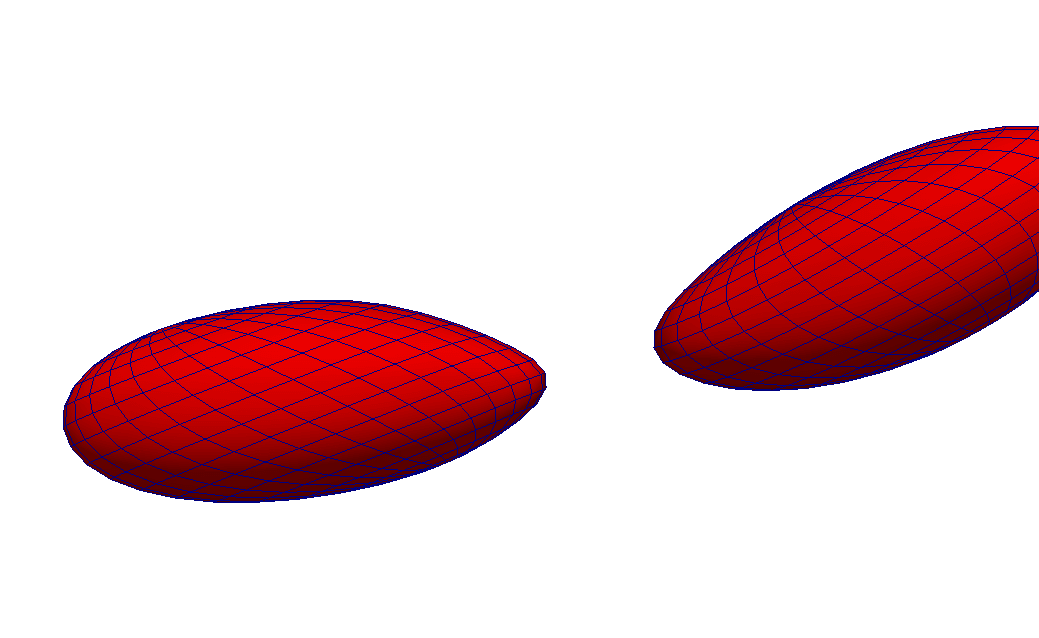
\includegraphics[width=52pt,height=35pt]{shear5}}}
%  \mcaption{fig:shear-snap}{}{Snapshots of two vesicles in shear flow.} \vspace{-5pt}
%    %At $T=0$, two vesicles are placed at $[-5.5, 0, 0]$ and $[0, 0, 0]$ respectively.}
%\end{figure}%
\begin{figure}[!htb]
  \centering
    \includepgf{conv}
    \mcaption{fig:shear-conv}{Temporal error convergence of shear flow simulation in \cref{fig:shear-snap}}{
    %The initial offset is $\delta_0 = 0$.
    Shown is the error in the final ($T=25$)
    centroid location as we decrease the time step size for two
    spherical harmonic orders $16$ and $32$. 
  We observe $O(\Delta t)$ convergence in time and hence the
  collission detection algorithm converges at the same order as the
  time stepper.}
    %As expected we observe first order convergence with
  %our time stepping scheme.  }
  \vspace{-5pt}
\end{figure}%
\subsection{High volume fraction}
The \rbc volume fraction, i.e., the ratio of volume occupied by \rbcs
compared to the overall blood volume is 36-48\% in healthy women and
40-54\% in healthy men \cite{billett1990hemoglobin}. As can be seen in the tables in
\cref{fig:wscale-large-grain,fig:wscale-knl}, the volume fraction in
our weak scaling simulations is below these values, which is mostly due to
the procedure used to fill the blood vessel with \rbcs (see the
discussion in \cref{ss:implementation}).
However, \rbc volume fractions in capillaries and small arteries is
known to be be around 10-20\%
\cite{wang2013simulation,saadat2019simulation}, which our scaling
simulations achieve.
To demonstrate that we can simulate even higher volume fraction blood flows,
\cref{fig:high-vol-snap} shows a test of 140 \rbcs sedimenting under a
gravitational force in a small capsule. The volume fraction for this example is
47\%, calculated by dividing the amount of volume occupied by \rbcs by the
volume of the capsule.
By the end of the simulation, we achieve a volume fraction
of 55\% in the lower part of the domain (determined by bounding the
\rbcs by a tighter cylinder than the original domain boundary) since
the \rbcs have become more tightly packed.
While such high volume fractions typically do not occur in capillary flow on average, in some scenarios (local fluctuations, sedimentation, microfluidics) these high concentrations need to be handled. 

